\chapter{\acrshort{mpi} Process Pinning}
\label{app:mm-mumps-process-pinning}


%\figpointer{\ref{fig:app-mumps-close-vs-spread-1}}
\begin{figure}[htpb]
\centering
	\begin{tabular}{cc}
		\subfloat[HW1 - k3-2]{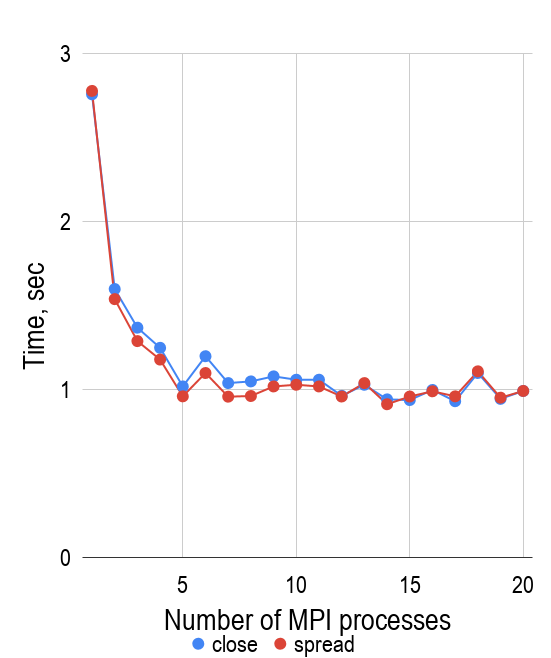
\includegraphics[width=0.48\textwidth]{figures/chapter-2/spread-vs-close/grs-cluster/k3-2.png}} &
		\subfloat[HW2 - k3-2]{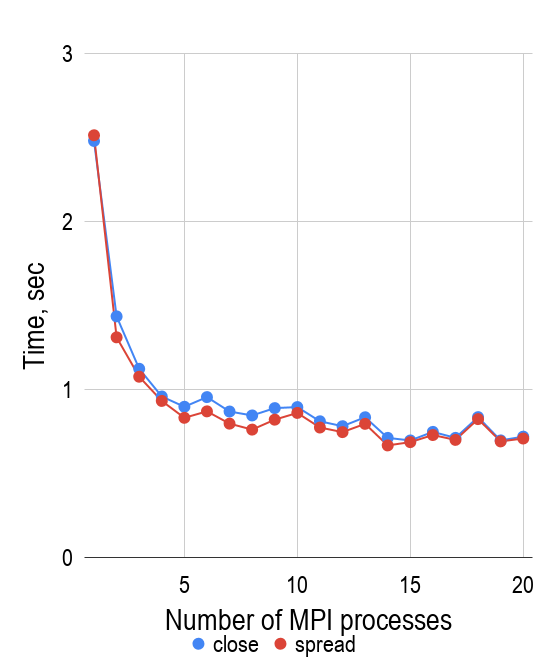
\includegraphics[width=0.48\textwidth]{figures/chapter-2/spread-vs-close/linux-cluster/k3-2.png}} \\
		\subfloat[HW1 - torso3]{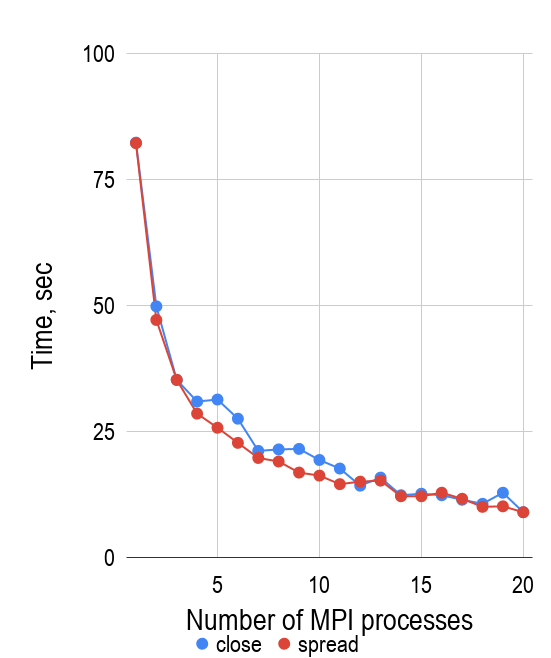
\includegraphics[width=0.48\textwidth]{figures/chapter-2/spread-vs-close/grs-cluster/torso3.png}} &
		\subfloat[HW2 - torso3]{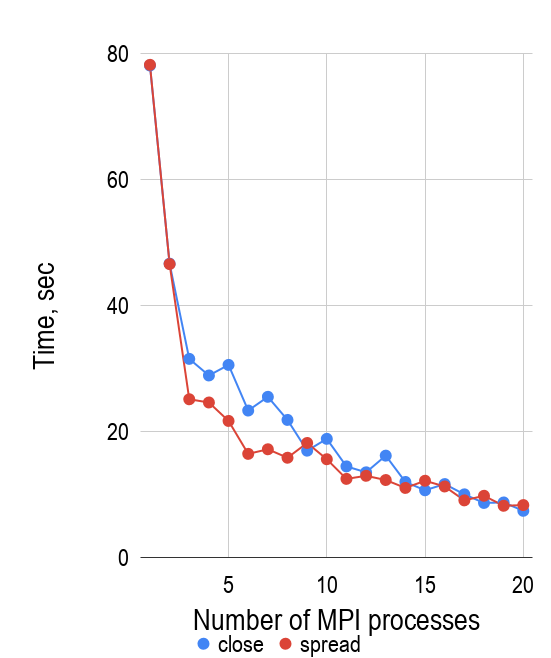
\includegraphics[width=0.48\textwidth]{figures/chapter-2/spread-vs-close/linux-cluster/torso3.png}} \\
	\end{tabular}
	\caption{Comparisons of \textit{close} and \textit{spread} pinning strategies applied to parallel factorizations of \textit{cube-64} and \textit{torso3} matrices}
	\label{fig:app-mumps-close-vs-spread-1}
\end{figure}


%\figpointer{\ref{fig:app-mumps-close-vs-spread-2}}
\begin{figure}[htpb]
\centering
	\begin{tabular}{cc}
		\subfloat[HW1 - consph]{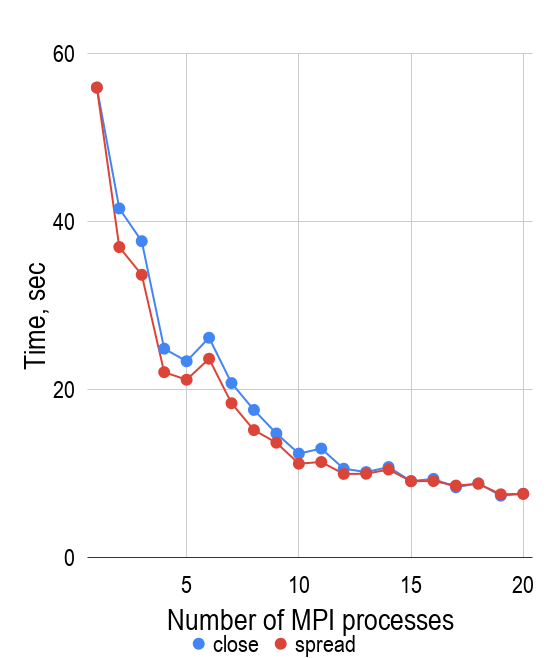
\includegraphics[width=0.48\textwidth]{figures/chapter-2/spread-vs-close/grs-cluster/consph.png}} &
		\subfloat[HW2 - consph]{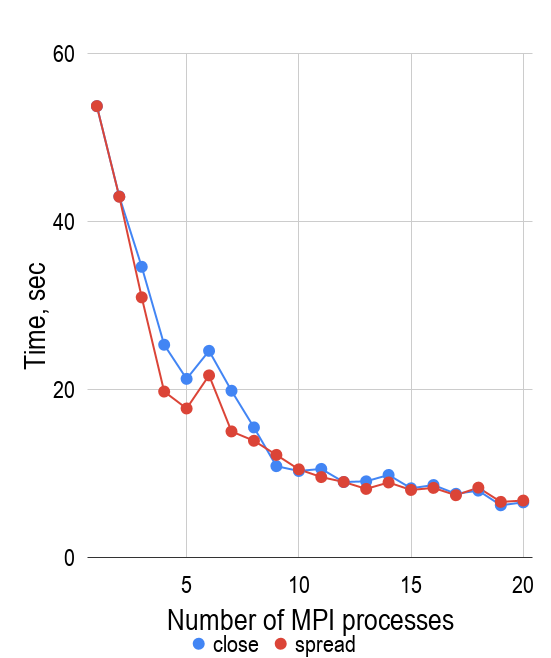
\includegraphics[width=0.48\textwidth]{figures/chapter-2/spread-vs-close/linux-cluster/consph.png}} \\
		\subfloat[HW1 - memchip\_3]{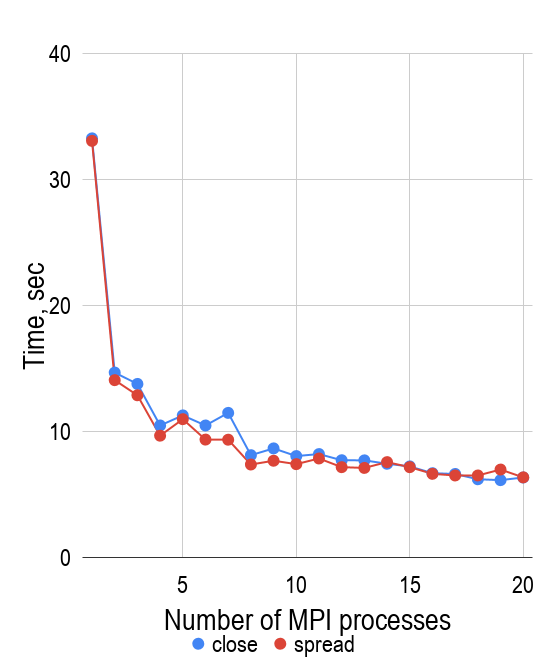
\includegraphics[width=0.48\textwidth]{figures/chapter-2/spread-vs-close/grs-cluster/memchip.png}} &
		\subfloat[HW2 - memchip]{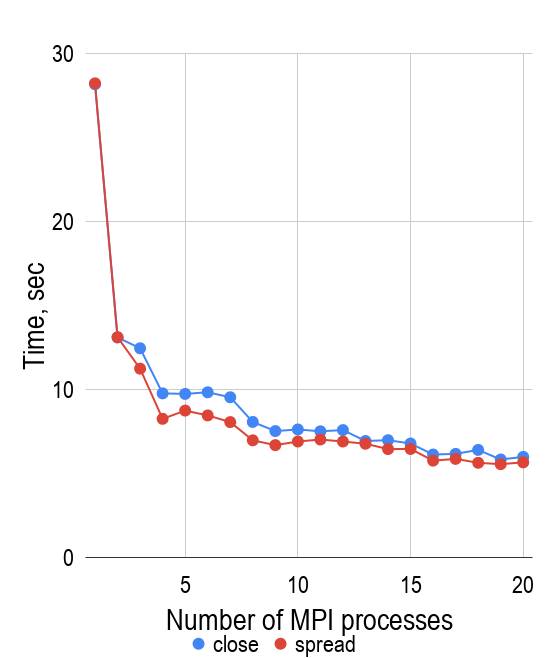
\includegraphics[width=0.48\textwidth]{figures/chapter-2/spread-vs-close/linux-cluster/memchip.png}} \\
	\end{tabular}
	\caption{Comparisons of \textit{close} and \textit{spread} pinning strategies applied to parallel factorizations of \textit{consph} and \textit{memchip} matrices}
	\label{fig:app-mumps-close-vs-spread-2}
\end{figure}

